As described in the System Requirements Document (SRD), the audio DSP must incorporate multiple input and output connectors. 

\begin{figure}[ht]
    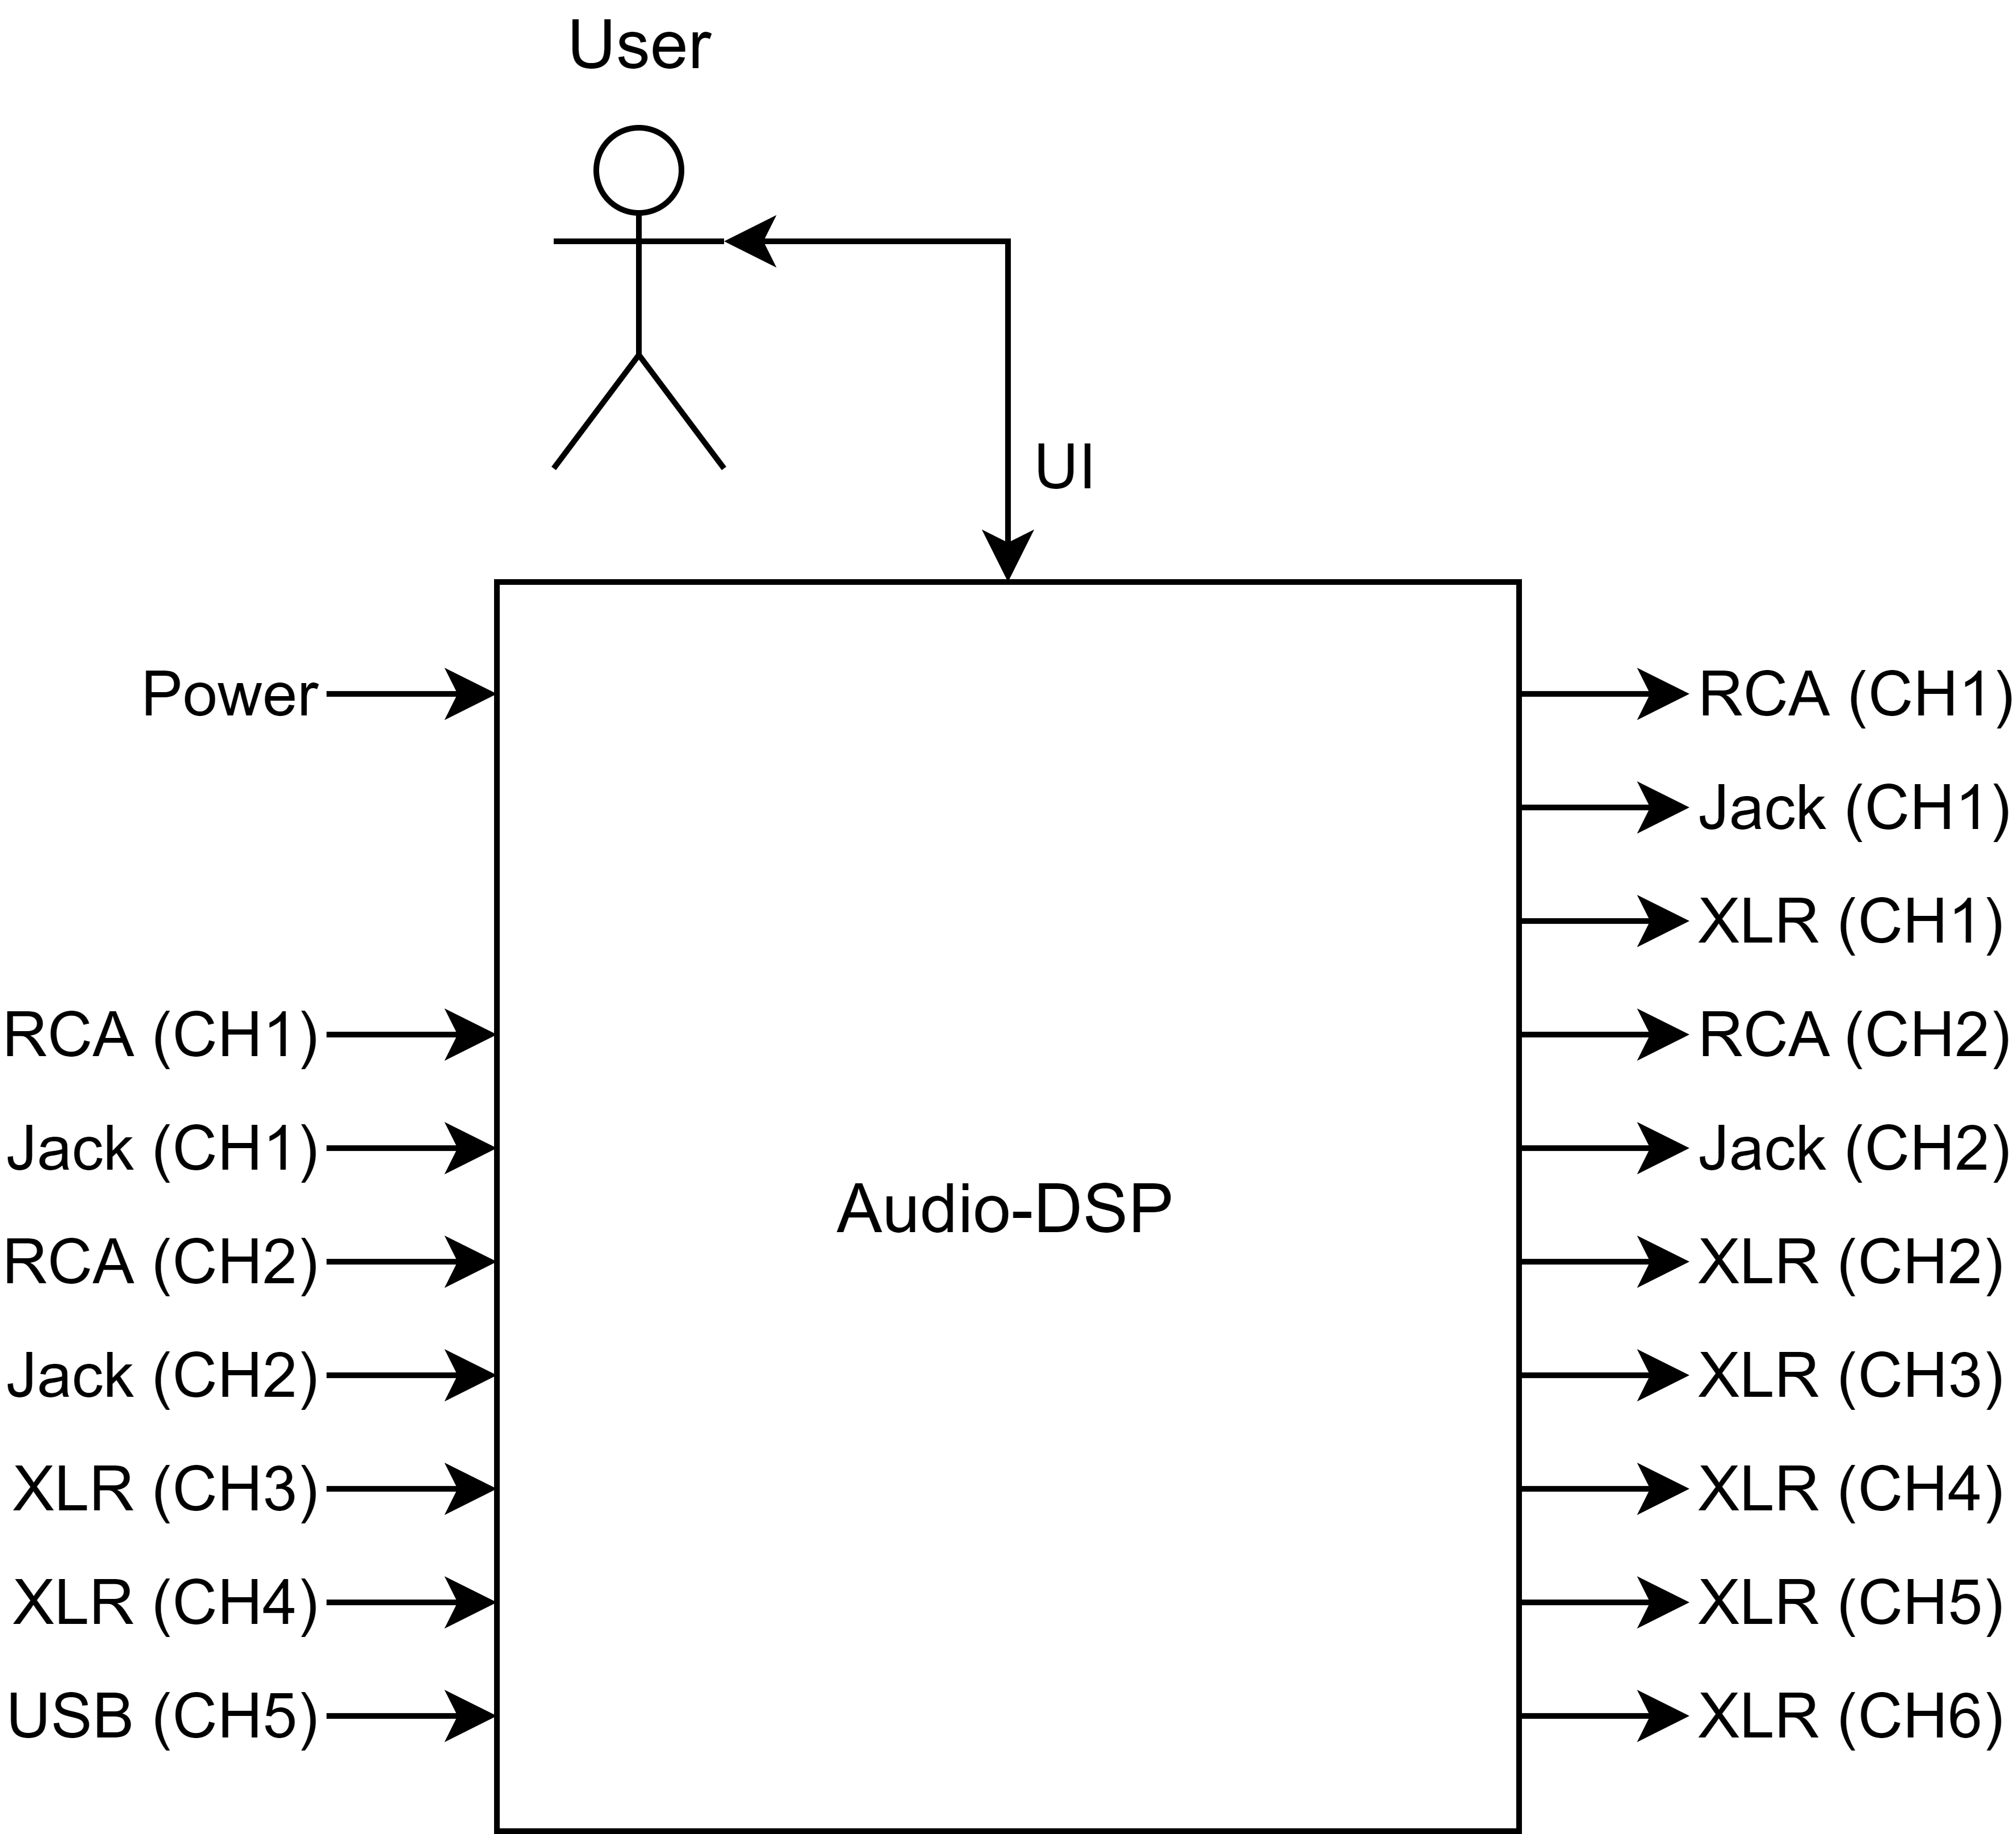
\includegraphics[width=\linewidth]{Black_box_representation.png}
    \caption{Black box representation}
    \label{fig:Black-box-rep}
\end{figure}

In figure \ref{fig:Black-box-rep} you see ........

\section{Inputs}
The system includes the following inputs:
\begin{itemize}
    \item DC jack to power the system
    \item CH1 RCA or jack
    \item CH2 RCA or jack
    \item CH3 XLR
    \item CH4 XLR
    \item CH5 USB (optional)
\end{itemize}

\section{Outputs}
Output channels 1 and 2 provide the most flexibility as each channel features a balanced XLR output as well as a parallel-connected RCA and jack input. Therefore, the RCA and jack input always carry precisely the same signal. Output channels 3 through 6 exclusively have balanced XLR outputs. The audio DSP, therefore, has the following outputs:

\begin{itemize}
    \item CH1 XLR, RCA and jack
    \item CH2 XLR, RCA and jack
    \item CH3 XLR
    \item CH4 XLR
    \item CH5 XLR
    \item CH6 XLR
\end{itemize}

\section{User interface}
